\documentclass[a4paper,12pt]{article}

% include headers and preamble for reoport
% file: includes-report.tex
% -----------------------------------------------------------------------------
% includes for studies report
% -----------------------------------------------------------------------------

\usepackage{amsmath}
\usepackage{setspace}
\usepackage[top=1.2in, bottom=1.2in]{geometry}
\usepackage[x11names]{xcolor}

\usepackage{float} % to force placement of images etc.

\usepackage{graphicx}
\usepackage[utf8]{inputenc}
\usepackage{siunitx}

% // -- for different section heading color --
\usepackage{sectsty}
\usepackage{xcolor}
% \chapterfont{\color{blue}}  % sets colour of chapters
% \definecolor{MyBlue}{rgb}{0.78,0.9,1} % rgb color code
% \definecolor{DarkBlue}{HTML}{002f4c} % HTML HEX color code
\definecolor{DarkBlue}{RGB}{0,47,76} % RGB color code
\sectionfont{\color{DarkBlue}}  % sets colour of sections
\subsectionfont{\color{DarkBlue}}  % sets colour of sections

\usepackage{float}


%\usepackage{multirow}
%\usepackage{pgfplots}
\usepackage{subcaption}

% // -- for source code listings --
\usepackage{color}
\definecolor{OliveGreen}{RGB}{0,128,0}
\usepackage{listings}
\usepackage{caption}
\DeclareCaptionFont{white}{\color{white}}
\DeclareCaptionFormat{listing}{\colorbox{gray}{\parbox{\textwidth}{#1#2#3}}}
\captionsetup[lstlisting]{format=listing,labelfont=white,textfont=white}


\lstdefinestyle{cStyle}{language=C}
\lstset{
language=C,
%basicstyle=\small\ttfamily,
basicstyle=\small\ttfamily,
keywordstyle=\color{blue}\ttfamily,
stringstyle=\color{red}\ttfamily,
commentstyle=\color{magenta}\ttfamily,
morecomment=[l][\color{magenta}]{\#},
numbers=left,
numberstyle=\tiny,
% frame=tb,
columns=fullflexible,
showstringspaces=false,
tabsize=2
}
\usepackage{matlab-prettifier}
\lstdefinestyle{matlabStyle}{language=matlab}
\lstset{
%style=Matlab-editor,
language=matlab,
%basicstyle=\small\ttfamily,
basicstyle=\small\ttfamily,
keywordstyle=\color{blue}\ttfamily,
stringstyle=\color{red}\ttfamily,
commentstyle=\color{OliveGreen}\ttfamily,
morecomment=[l][\color{OliveGreen}]{\#},
numbers=left,
numberstyle=\tiny,
% frame=tb,
columns=fullflexible,
showstringspaces=false,
tabsize=2
}
\lstdefinestyle{vhdlStyle}{language=vhdl}
\lstset{
language=vhdl,
%basicstyle=\small\ttfamily,
basicstyle=\small\ttfamily,
keywordstyle=\color{blue}\ttfamily,
stringstyle=\color{red}\ttfamily,
commentstyle=\color{magenta}\ttfamily,
morecomment=[l][\color{magenta}]{\#},
numbers=left,
numberstyle=\tiny,
% frame=tb,
columns=fullflexible,
showstringspaces=false,
tabsize=2
}

% bibliography (Literaturverzeinis)
\usepackage[round]{natbib}
\bibliographystyle{alphadin} % set format

% // -- source code listings --


\title{Bachelorprojekt}
\date{2018-11-21}
\author{Fabian Huber}

\begin{document}

% Titlepage for HAW lab report
\begin{titlepage}
\definecolor{blue(ncs)}{rgb}{0.0, 0.53, 0.74}
\begin{figure}[h!]
  \begin{flushright}
  \begin{spacing}{1.5}
  
\includegraphics[width=.5\linewidth]{images/hawlogo.png}
  \label{fig:hawlogo}\\
  \small Fakultät Technik und Informatik\\
  \small Department Informations- und Elektrotechnik
  \end{spacing}
  \end{flushright}
\end{figure}
\textbf{\large Bachelorprojekt}
\begin{center}\noindent\textcolor{blue(ncs)}{\rule{13.5cm}{0.5mm}}\end{center}
\begin{spacing}{4.5}
\textbf{\huge Automated Driving}
\end{spacing}
\textbf{\large\indent RC Car Control with Open Source Image Processing}
\begin{center}\noindent\textcolor{blue(ncs)}{\rule{13.5cm}{0.5mm}}\end{center}
\begin{spacing}{1.15}
\vspace*{\fill}
\noindent
\textnormal{\\
  Prof. Dr.-Ing. Marc Hensel \\
  \textbf{Projektgruppe:} Fabian Huber, Enzo Morino, Markus Trockel \\
  \textbf{Abgabe:} DD.MM.2019 \\
}
\end{spacing}
\end{titlepage}
% --- end of titlepage ---

  \pagenumbering{gobble}
  \newpage

  \tableofcontents
  \newpage

  \pagenumbering{arabic}

  \section{Einleitung}
    \ \\

  \section{Ziel des Projekts}
    \ \\
    
    Ziel des Projekts ist es, ein Modell-Auto zu bauen bzw. zu programmieren, das mithilfe eines Raspberry Pi's und einer Kamera autonom zwischen zwei Fahrbahnlinien die Spur halten kann. Das Auto soll auf einer 4 Meter langen geraden Strecke auf der Fahrbahn bleiben, einer Rechts- und einer Linkskurve mit angemessen großem Radius um 90° folgen, und eine Kreisfahrt in beide Richtungen beherrschen können. Optional soll auch eine 8-förmige Strecke wie beim Carolo-Cup befahren werden.
  
  \section{Kurzübersicht}
    \ \\
    
    
  \section{Prinzip der Steuerung}
  	\ \\
  	
  Über ein Python-Programm, welches auf dem Raspberry Pi läuft, wird der Video-Stream der angeschlossenen Kamera iterativ ausgewertet. Es werden die beiden Fahrbahnlinien erkannt, durch Geraden angenähert und deren Fluchtpunkt berechnet. Auf Grundlage der x-Koordinate dieses Fluchtpunktes wird ein Ausgangssignal berechnet, welches über das PWM-Modul den Servo ansteuert, und damit den Lenkwinkel festlegt.  
  	

  \section{Hardware}
    \ \\
    \subsection{Raspberry Pi 3}
    \ \\
    \subsection{Motorcontroller}
    \ \\
    \subsection{Ultraschallsensor}
    \ \\
    \subsection{RC Fahrzeug}
    \ \\
  
  \section{Software}
    \ \\
    \subsection{Aufbau}
    \ \\
    \begin{minipage}{\columnwidth}
      \makeatletter
      \def\@captype{figure}
      \makeatother
      \centering
      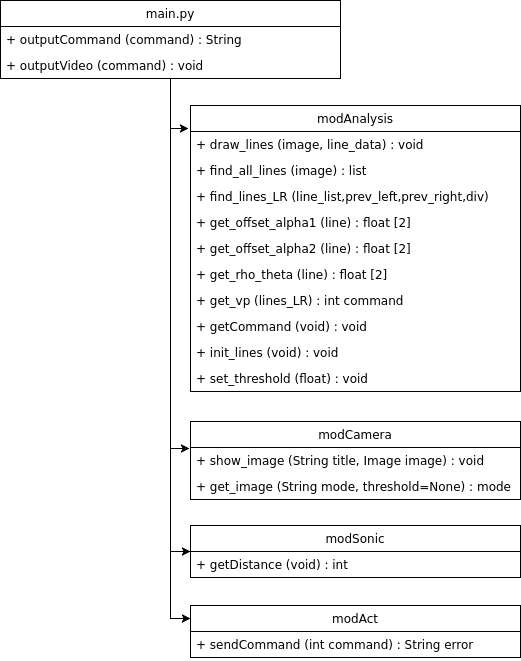
\includegraphics[width=0.8\linewidth]{images/code-flowchart.png}
      \caption{Aufbau des Python Codes}
      \label{fig:image-01}
    \end{minipage}
    \ \\

    \subsection{Externe Module}
    \ \\
    \begin{minipage}{\columnwidth}
      \makeatletter
      \def\@captype{table}
      \makeatother
      \centering
      %\rowcolors{1}{grey}{white}
      \begin{tabular}{ l | l }
      % \multicolumn{2}{|c}{Frame \#} & \multicolumn{4}{|c}{LCD 0/3} &
      Name & Beschreibung \\ \hline \hline
      tkinter & ... \\
      Adafruit\_PCA9685 & Bibliothek zur Ansteuerung des Motorcontrollers \\
      numpy & Bibliothek zur Verwendung von Matlab Funktionen \\
      cv2 & OpenCV 2 bietet Algorithmen zur Bildverarbeitung \\
      io & ... \\
      time & ... \\
      importlib & ... \\
      argparse & ... \\
      pivideostream & ... \\
      picamera & ... \\
      threading & ... \\
      RPi.GPIO & Bibliothek zur Ansteuerung der GPIO ports des Raspbery Pi \\
      \end{tabular}
      \caption{verwendete externe Python Module}
      \label{tab:01}
    \end{minipage}
    
    \subsection{Eigene Module}
    \ \\
    \begin{minipage}{\columnwidth}
      \makeatletter
      \def\@captype{table}
      \makeatother
      \centering
      %\rowcolors{1}{grey}{white}
      \begin{tabular}{ l | l }
      % \multicolumn{2}{|c}{Frame \#} & \multicolumn{4}{|c}{LCD 0/3} &
      Name & Beschreibung \\ \hline \hline
      modAnalysis & Verantwortlich für die eigentliche Verarbeitung der visuellen Informationen \\
      modAct & Verantwortlich für die Ansteuerung des Motors und der Lenkung \\
      modCamera & Bereitet das Kamerabild für die Verarbeitung und Anzeige vor. \\
      modSonic & Kommuniziert mit dem Ultraschallsensor und liefert Distanz zum Hindernis.\\
      \end{tabular}
      \caption{verwendete eigene Python Module}
      \label{tab:01}
    \end{minipage}

	\subsection{Verwendete Repräsentationen von Geraden}

	\subsection{Auswertung des Kamerabildes}	

	Das Bild der Kamera wird iterativ ausgewertet um die beiden Fahrbahnlinien zu erkennen und daraus ein Ausgangssignal für die Steuerung zu generieren. Die Fahrbahnlinien werden durch zwei Geraden angenähert. \\ 
	Beim Start des Programms werden für die beiden Geraden feste Werte vorgegeben. Anhand dieser Anfangswerte werden die im nächsten Durchlauf die Fahrbahnlinien durch bessere Werte angenähert.\\
	Dafür wird das Bild zunächst mithilfe eines Schwellwertes in Schwarzweiß umgewandelt. Bei einem geeigneten Schwellwert sollten nun möglichst nur die beiden Fahrbahnlinien weiß sein (den Wert 1 haben).\\
	Als nächstes wird die Funktion HoughLines aus der Bibliothek cv ausgeführt, die alle Geraden im Bild sucht. Die Funktion Houghlines gibt als Rückgabewert eine Liste von Geraden zurück, die in Polarkoordinaten durch einen Winkel $\rho$ und eine Steigung $\theta$ rerpäsentiert werden. $\rho$ ist der Winkel zwischen der Normalen, die senkrecht auf der Geraden steht, und der x-Achse. $\theta$ ist die Länge dieser Normalen, d.h. der Abstand zwischen der Geraden und dem Ursprung des Koordinatensystems.


  % \bibliography{hawey-documentation}
  % \bibliographystyle{ieeetr}

\end{document}
